\documentclass[../../../../main.tex]{subfiles}
\begin{document}

図は $O$ を中心とする四分円であって，$OA=\sqrt3$，$OB=1$ である。
いま，動点 $P$ が円弧に沿って $A$ から $Q$ まで進み，さらに $Q$ から $B$ まで直進する。
ところが，$P$ の弧 $AQ$ 上での速さは 2，線分 $QB$ 上での速さは 1 である。
この路に沿っての $A$ から $B$ までの所要時間が最小となるような点 $Q$ の位置を定めよ。

\begin{figure}[htbp]
  \centering
  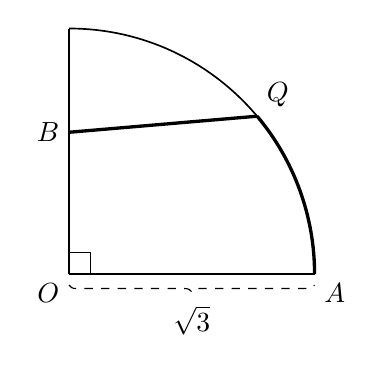
\begin{tikzpicture}[scale=1.8, >=stealth]
    \def\r{1.732}
    \coordinate (O) at (0,0);
    \coordinate (A) at (\r,0);
    \coordinate (B) at (0,1);
    \coordinate (Q) at (40:\r);
    \coordinate (Top) at (0,\r);

    \draw[line width=0.6pt] (Top) arc (90:0:\r);
    \draw[line width=0.6pt] (O) -- (Top);
    \draw[line width=0.6pt] (O) -- (A);

    % 経路 A -> Q -> B (太線)
    \draw[very thick] (A) arc (0:40:\r);
    \draw[very thick] (Q) -- (B);

    % 直角マーク
    \draw (0.15,0) -- (0.15,0.15) -- (0,0.15);

    \node[below left] at (O) {$O$};
    \node[below right] at (A) {$A$};
    \node[left] at (B) {$B$};
    \node[above right] at (Q) {$Q$};

    % 寸法ラベル sqrt(3)
    \draw[dashed, decorate, decoration={brace, mirror, raise=4pt}] (O) -- (A) node[midway, below=8pt] {$\sqrt{3}$};
  \end{tikzpicture}
\end{figure}

\end{document}
